\documentclass[twoside]{book}

% Packages required by doxygen
\usepackage{fixltx2e}
\usepackage{calc}
\usepackage{doxygen}
\usepackage[export]{adjustbox} % also loads graphicx
\usepackage{graphicx}
\usepackage[utf8]{inputenc}
\usepackage{makeidx}
\usepackage{multicol}
\usepackage{multirow}
\PassOptionsToPackage{warn}{textcomp}
\usepackage{textcomp}
\usepackage[nointegrals]{wasysym}
\usepackage[table]{xcolor}

% Font selection
\usepackage[T1]{fontenc}
\usepackage[scaled=.90]{helvet}
\usepackage{courier}
\usepackage{amssymb}
\usepackage{sectsty}
\renewcommand{\familydefault}{\sfdefault}
\allsectionsfont{%
  \fontseries{bc}\selectfont%
  \color{darkgray}%
}
\renewcommand{\DoxyLabelFont}{%
  \fontseries{bc}\selectfont%
  \color{darkgray}%
}
\newcommand{\+}{\discretionary{\mbox{\scriptsize$\hookleftarrow$}}{}{}}

% Page & text layout
\usepackage{geometry}
\geometry{%
  a4paper,%
  top=2.5cm,%
  bottom=2.5cm,%
  left=2.5cm,%
  right=2.5cm%
}
\tolerance=750
\hfuzz=15pt
\hbadness=750
\setlength{\emergencystretch}{15pt}
\setlength{\parindent}{0cm}
\setlength{\parskip}{3ex plus 2ex minus 2ex}
\makeatletter
\renewcommand{\paragraph}{%
  \@startsection{paragraph}{4}{0ex}{-1.0ex}{1.0ex}{%
    \normalfont\normalsize\bfseries\SS@parafont%
  }%
}
\renewcommand{\subparagraph}{%
  \@startsection{subparagraph}{5}{0ex}{-1.0ex}{1.0ex}{%
    \normalfont\normalsize\bfseries\SS@subparafont%
  }%
}
\makeatother

% Headers & footers
\usepackage{fancyhdr}
\pagestyle{fancyplain}
\fancyhead[LE]{\fancyplain{}{\bfseries\thepage}}
\fancyhead[CE]{\fancyplain{}{}}
\fancyhead[RE]{\fancyplain{}{\bfseries\leftmark}}
\fancyhead[LO]{\fancyplain{}{\bfseries\rightmark}}
\fancyhead[CO]{\fancyplain{}{}}
\fancyhead[RO]{\fancyplain{}{\bfseries\thepage}}
\fancyfoot[LE]{\fancyplain{}{}}
\fancyfoot[CE]{\fancyplain{}{}}
\fancyfoot[RE]{\fancyplain{}{\bfseries\scriptsize Generated by Doxygen }}
\fancyfoot[LO]{\fancyplain{}{\bfseries\scriptsize Generated by Doxygen }}
\fancyfoot[CO]{\fancyplain{}{}}
\fancyfoot[RO]{\fancyplain{}{}}
\renewcommand{\footrulewidth}{0.4pt}
\renewcommand{\chaptermark}[1]{%
  \markboth{#1}{}%
}
\renewcommand{\sectionmark}[1]{%
  \markright{\thesection\ #1}%
}

% Indices & bibliography
\usepackage{natbib}
\usepackage[titles]{tocloft}
\setcounter{tocdepth}{3}
\setcounter{secnumdepth}{5}
\makeindex

% Hyperlinks (required, but should be loaded last)
\usepackage{ifpdf}
\ifpdf
  \usepackage[pdftex,pagebackref=true]{hyperref}
\else
  \usepackage[ps2pdf,pagebackref=true]{hyperref}
\fi
\hypersetup{%
  colorlinks=true,%
  linkcolor=blue,%
  citecolor=blue,%
  unicode%
}

% Custom commands
\newcommand{\clearemptydoublepage}{%
  \newpage{\pagestyle{empty}\cleardoublepage}%
}

\usepackage{caption}
\captionsetup{labelsep=space,justification=centering,font={bf},singlelinecheck=off,skip=4pt,position=top}

%===== C O N T E N T S =====

\begin{document}

% Titlepage & ToC
\hypersetup{pageanchor=false,
             bookmarksnumbered=true,
             pdfencoding=unicode
            }
\pagenumbering{roman}
\begin{titlepage}
\vspace*{7cm}
\begin{center}%
{\Large Toxic comment classificator }\\
\vspace*{1cm}
{\large Generated by Doxygen 1.8.11}\\
\end{center}
\end{titlepage}
\clearemptydoublepage
\tableofcontents
\clearemptydoublepage
\pagenumbering{arabic}
\hypersetup{pageanchor=true}

%--- Begin generated contents ---
\chapter{Module Index}
\section{Modules}
Here is a list of all modules\+:\begin{DoxyCompactList}
\item \contentsline{section}{Сокращения}{\pageref{group__aliases}}{}
\end{DoxyCompactList}

\chapter{Namespace Index}
\section{Пространства имен}
Полный список документированных пространств имен.\begin{DoxyCompactList}
\item\contentsline{section}{\mbox{\hyperlink{namespacetcc}{tcc}} \\*Пространство имен tcc }{\pageref{namespacetcc}}{}
\end{DoxyCompactList}

\chapter{Hierarchical Index}
\section{Иерархия классов}
Иерархия классов.\begin{DoxyCompactList}
\item \contentsline{section}{Controller}{\pageref{class_controller}}{}
\begin{DoxyCompactList}
\item \contentsline{section}{Main\+Controller}{\pageref{class_main_controller}}{}
\end{DoxyCompactList}
\item \contentsline{section}{Core}{\pageref{class_core}}{}
\item \contentsline{section}{Data\+Processing}{\pageref{class_data_processing}}{}
\item \contentsline{section}{Data\+Provider}{\pageref{class_data_provider}}{}
\begin{DoxyCompactList}
\item \contentsline{section}{File\+Data\+Provider}{\pageref{class_file_data_provider}}{}
\end{DoxyCompactList}
\item \contentsline{section}{Message}{\pageref{class_message}}{}
\end{DoxyCompactList}

\chapter{Class Index}
\section{Классы}
Классы с их кратким описанием.\begin{DoxyCompactList}
\item\contentsline{section}{\mbox{\hyperlink{class_controller}{Controller}} \\*Интерфейс для классов контроллеров управляющими ходом программы }{\pageref{class_controller}}{}
\item\contentsline{section}{\mbox{\hyperlink{class_core}{Core}} \\*Интерфейс классов ядра для определения \char`\"{}недоброжелательности\char`\"{} текста }{\pageref{class_core}}{}
\item\contentsline{section}{\mbox{\hyperlink{class_data_processing}{Data\+Processing}} \\*Интерфейс для классов предобработки текста }{\pageref{class_data_processing}}{}
\item\contentsline{section}{\mbox{\hyperlink{class_data_provider}{Data\+Provider}} \\*Интерфейс для классов считывания/записи данных }{\pageref{class_data_provider}}{}
\item\contentsline{section}{\mbox{\hyperlink{class_file_data_provider}{File\+Data\+Provider}} \\*Класс для считывания/записи данных из/в файл(а) }{\pageref{class_file_data_provider}}{}
\item\contentsline{section}{\mbox{\hyperlink{class_main_controller}{Main\+Controller}} \\*Основной класс контроллер управляющий ходом программы }{\pageref{class_main_controller}}{}
\item\contentsline{section}{\mbox{\hyperlink{class_message}{Message}} }{\pageref{class_message}}{}
\end{DoxyCompactList}

\chapter{Module Documentation}
\hypertarget{group__aliases}{}\section{Сокращения}
\label{group__aliases}\index{Сокращения@{Сокращения}}
\subsection*{Typedefs}
\begin{DoxyCompactItemize}
\item 
using \hyperlink{group__aliases_gae00908f082db728f73e52c3b4932261a}{tcc\+::uint} = unsigned int\hypertarget{group__aliases_gae00908f082db728f73e52c3b4932261a}{}\label{group__aliases_gae00908f082db728f73e52c3b4932261a}

\begin{DoxyCompactList}\small\item\em Положительное целое \end{DoxyCompactList}\item 
using \hyperlink{group__aliases_ga33d75c4fd4f8d49a28f246c2e0a0f3a5}{tcc\+::vec} = std\+::vector$<$ uint $>$\hypertarget{group__aliases_ga33d75c4fd4f8d49a28f246c2e0a0f3a5}{}\label{group__aliases_ga33d75c4fd4f8d49a28f246c2e0a0f3a5}

\begin{DoxyCompactList}\small\item\em Вектор положительных целых \end{DoxyCompactList}\item 
using \hyperlink{group__aliases_ga085c5ca5bf5645ff17c0ede30f56b08f}{tcc\+::text} = std\+::vector$<$ std\+::string $>$\hypertarget{group__aliases_ga085c5ca5bf5645ff17c0ede30f56b08f}{}\label{group__aliases_ga085c5ca5bf5645ff17c0ede30f56b08f}

\begin{DoxyCompactList}\small\item\em Массив текстов \end{DoxyCompactList}\end{DoxyCompactItemize}


\subsection{Detailed Description}
Сокращения для названий используемых типов 
\chapter{Namespace Documentation}
\hypertarget{namespacetcc}{}\section{Пространство имен tcc}
\label{namespacetcc}\index{tcc@{tcc}}


Пространство имен tcc.  


\subsection*{Классы}
\begin{DoxyCompactItemize}
\item 
class \mbox{\hyperlink{classtcc_1_1_controller}{Controller}}
\begin{DoxyCompactList}\small\item\em Интерфейс для классов контроллеров управляющими ходом программы \end{DoxyCompactList}\item 
class \mbox{\hyperlink{classtcc_1_1_core}{Core}}
\begin{DoxyCompactList}\small\item\em Интерфейс классов ядра для классификации \char`\"{}недоброжелательности\char`\"{} текста \end{DoxyCompactList}\item 
class \mbox{\hyperlink{classtcc_1_1_data_processing}{Data\+Processing}}
\begin{DoxyCompactList}\small\item\em Интерфейс для классов предобработки текста \end{DoxyCompactList}\item 
class \mbox{\hyperlink{classtcc_1_1_data_provider}{Data\+Provider}}
\begin{DoxyCompactList}\small\item\em Интерфейс для классов считывания/записи данных \end{DoxyCompactList}\item 
class \mbox{\hyperlink{classtcc_1_1_file_data_provider}{File\+Data\+Provider}}
\begin{DoxyCompactList}\small\item\em Класс для считывания/записи данных из/в файл(а) \end{DoxyCompactList}\item 
class \mbox{\hyperlink{classtcc_1_1_main_controller}{Main\+Controller}}
\begin{DoxyCompactList}\small\item\em Основной класс контроллер управляющий ходом программы \end{DoxyCompactList}\item 
class \mbox{\hyperlink{classtcc_1_1_message}{Message}}
\item 
class \mbox{\hyperlink{classtcc_1_1_random_core}{Random\+Core}}
\begin{DoxyCompactList}\small\item\em Класс -\/ ядро для классификации \char`\"{}недоброжелательности\char`\"{} текста \end{DoxyCompactList}\end{DoxyCompactItemize}


\subsection{Подробное описание}
Пространство имен tcc. 

namespace tcc 
\hypertarget{namespace_ui}{}\section{Ui Namespace Reference}
\label{namespace_ui}\index{Ui@{Ui}}


Пространство имён \hyperlink{namespace_ui}{Ui}, используемое объектами графического интерфейса  




\subsection{Detailed Description}
Пространство имён \hyperlink{namespace_ui}{Ui}, используемое объектами графического интерфейса 

namespace \hyperlink{namespace_ui}{Ui} 
\chapter{Class Documentation}
\hypertarget{classtcc_1_1_b_o_w}{}\section{tcc\+:\+:B\+OW Class Reference}
\label{classtcc_1_1_b_o_w}\index{tcc\+::\+B\+OW@{tcc\+::\+B\+OW}}


Класс для хранения информации о корпусе слов в виде мешка слов  




{\ttfamily \#include $<$B\+O\+W.\+h$>$}

\subsection*{Public Member Functions}
\begin{DoxyCompactItemize}
\item 
\hyperlink{classtcc_1_1_b_o_w_add04201669428662c6446d6d6dfb390c}{B\+OW} (\hyperlink{namespacetcc_a9bdf9e81347b7904a6a7f8427d6465dc}{text\+Vec} \&texts)
\begin{DoxyCompactList}\small\item\em Конструктор экземпляра класса \end{DoxyCompactList}\item 
void \hyperlink{classtcc_1_1_b_o_w_aa46799ba0df5171e704c0d633c498d04}{add\+\_\+word} (std\+::string \&s)
\begin{DoxyCompactList}\small\item\em Добавление слова в словарь \end{DoxyCompactList}\item 
\hyperlink{group__aliases_gae00908f082db728f73e52c3b4932261a}{uint} \hyperlink{classtcc_1_1_b_o_w_a59df3d61c19022ddad6232945eec37ff}{find\+\_\+word} (std\+::string \&s)
\begin{DoxyCompactList}\small\item\em Поиск информации о слове \end{DoxyCompactList}\end{DoxyCompactItemize}


\subsection{Detailed Description}
Класс для хранения информации о корпусе слов в виде мешка слов 

\subsection{Constructor \& Destructor Documentation}
\index{tcc\+::\+B\+OW@{tcc\+::\+B\+OW}!B\+OW@{B\+OW}}
\index{B\+OW@{B\+OW}!tcc\+::\+B\+OW@{tcc\+::\+B\+OW}}
\subsubsection[{\texorpdfstring{B\+O\+W(text\+Vec \&texts)}{BOW(textVec &texts)}}]{\setlength{\rightskip}{0pt plus 5cm}tcc\+::\+B\+O\+W\+::\+B\+OW (
\begin{DoxyParamCaption}
\item[{{\bf text\+Vec} \&}]{texts}
\end{DoxyParamCaption}
)}\hypertarget{classtcc_1_1_b_o_w_add04201669428662c6446d6d6dfb390c}{}\label{classtcc_1_1_b_o_w_add04201669428662c6446d6d6dfb390c}


Конструктор экземпляра класса 


\begin{DoxyParams}{Parameters}
{\em texts} & -\/ корпус текстов, на основе которых будет составлен мешок слов \\
\hline
\end{DoxyParams}


\subsection{Member Function Documentation}
\index{tcc\+::\+B\+OW@{tcc\+::\+B\+OW}!add\+\_\+word@{add\+\_\+word}}
\index{add\+\_\+word@{add\+\_\+word}!tcc\+::\+B\+OW@{tcc\+::\+B\+OW}}
\subsubsection[{\texorpdfstring{add\+\_\+word(std\+::string \&s)}{add_word(std::string &s)}}]{\setlength{\rightskip}{0pt plus 5cm}void tcc\+::\+B\+O\+W\+::add\+\_\+word (
\begin{DoxyParamCaption}
\item[{std\+::string \&}]{s}
\end{DoxyParamCaption}
)}\hypertarget{classtcc_1_1_b_o_w_aa46799ba0df5171e704c0d633c498d04}{}\label{classtcc_1_1_b_o_w_aa46799ba0df5171e704c0d633c498d04}


Добавление слова в словарь 


\begin{DoxyParams}{Parameters}
{\em s} & -\/ строка, содержащая слово \\
\hline
\end{DoxyParams}
\index{tcc\+::\+B\+OW@{tcc\+::\+B\+OW}!find\+\_\+word@{find\+\_\+word}}
\index{find\+\_\+word@{find\+\_\+word}!tcc\+::\+B\+OW@{tcc\+::\+B\+OW}}
\subsubsection[{\texorpdfstring{find\+\_\+word(std\+::string \&s)}{find_word(std::string &s)}}]{\setlength{\rightskip}{0pt plus 5cm}{\bf uint} tcc\+::\+B\+O\+W\+::find\+\_\+word (
\begin{DoxyParamCaption}
\item[{std\+::string \&}]{s}
\end{DoxyParamCaption}
)}\hypertarget{classtcc_1_1_b_o_w_a59df3d61c19022ddad6232945eec37ff}{}\label{classtcc_1_1_b_o_w_a59df3d61c19022ddad6232945eec37ff}


Поиск информации о слове 


\begin{DoxyParams}{Parameters}
{\em s} & -\/ искомое слово \\
\hline
\end{DoxyParams}
\begin{DoxyReturn}{Returns}
количество раз, когда слово встретилось в корпусе текстов 
\end{DoxyReturn}


The documentation for this class was generated from the following file\+:\begin{DoxyCompactItemize}
\item 
src/\+Classification/B\+O\+W.\+h\end{DoxyCompactItemize}

\hypertarget{classtcc_1_1_b_o_w_features}{}\section{tcc\+:\+:B\+O\+W\+Features Class Reference}
\label{classtcc_1_1_b_o_w_features}\index{tcc\+::\+B\+O\+W\+Features@{tcc\+::\+B\+O\+W\+Features}}


Преобразование на основе bag-\/of-\/words.  




{\ttfamily \#include $<$Vocab.\+h$>$}

Inheritance diagram for tcc\+:\+:B\+O\+W\+Features\+:\begin{figure}[H]
\begin{center}
\leavevmode
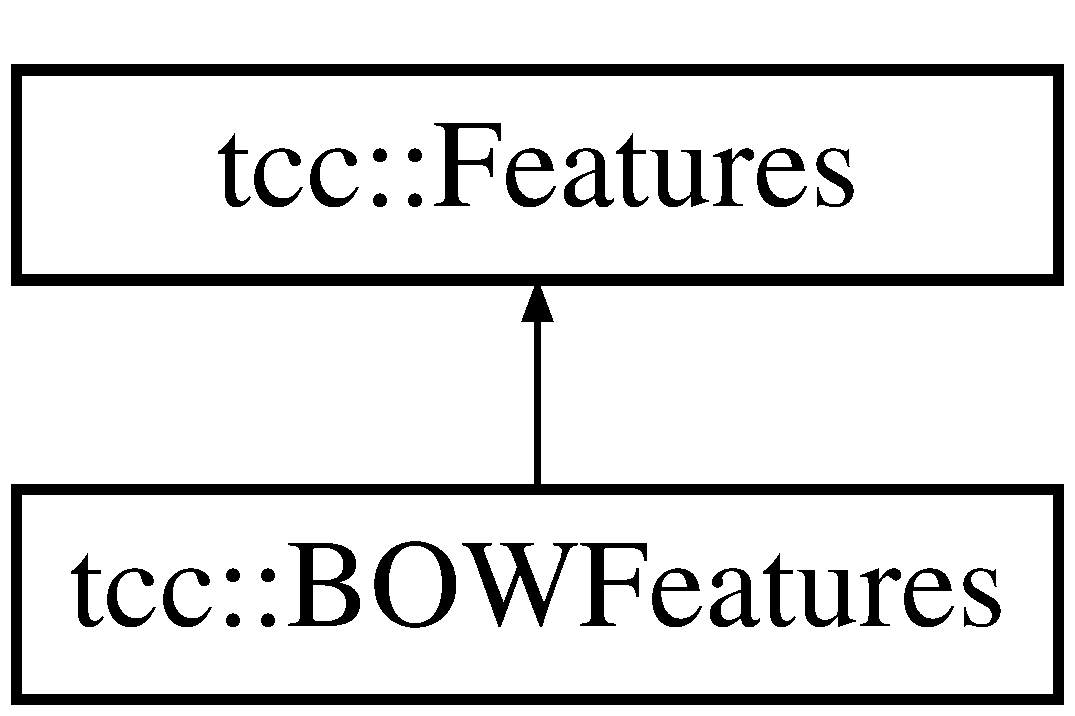
\includegraphics[height=2.000000cm]{classtcc_1_1_b_o_w_features}
\end{center}
\end{figure}
\subsection*{Public Member Functions}
\begin{DoxyCompactItemize}
\item 
\hyperlink{classtcc_1_1_b_o_w_features_a844e3c3dc3bd949c967d88cd695f41e5}{B\+O\+W\+Features} (std\+::shared\+\_\+ptr$<$ \hyperlink{classtcc_1_1_b_o_w}{B\+OW} $>$ global)
\begin{DoxyCompactList}\small\item\em Конструктор экземпляра класса \end{DoxyCompactList}\end{DoxyCompactItemize}


\subsection{Detailed Description}
Преобразование на основе bag-\/of-\/words. 

\subsection{Constructor \& Destructor Documentation}
\index{tcc\+::\+B\+O\+W\+Features@{tcc\+::\+B\+O\+W\+Features}!B\+O\+W\+Features@{B\+O\+W\+Features}}
\index{B\+O\+W\+Features@{B\+O\+W\+Features}!tcc\+::\+B\+O\+W\+Features@{tcc\+::\+B\+O\+W\+Features}}
\subsubsection[{\texorpdfstring{B\+O\+W\+Features(std\+::shared\+\_\+ptr$<$ B\+O\+W $>$ global)}{BOWFeatures(std::shared_ptr< BOW > global)}}]{\setlength{\rightskip}{0pt plus 5cm}tcc\+::\+B\+O\+W\+Features\+::\+B\+O\+W\+Features (
\begin{DoxyParamCaption}
\item[{std\+::shared\+\_\+ptr$<$ {\bf B\+OW} $>$}]{global}
\end{DoxyParamCaption}
)\hspace{0.3cm}{\ttfamily [inline]}}\hypertarget{classtcc_1_1_b_o_w_features_a844e3c3dc3bd949c967d88cd695f41e5}{}\label{classtcc_1_1_b_o_w_features_a844e3c3dc3bd949c967d88cd695f41e5}


Конструктор экземпляра класса 


\begin{DoxyParams}{Parameters}
{\em global} & -\/ информация о словах, встречающихся в корпусе текстов \\
\hline
\end{DoxyParams}


The documentation for this class was generated from the following file\+:\begin{DoxyCompactItemize}
\item 
src/\+Classification/Vocab.\+h\end{DoxyCompactItemize}

\hypertarget{classtcc_1_1_classifyer}{}\section{tcc\+:\+:Classifyer Class Reference}
\label{classtcc_1_1_classifyer}\index{tcc\+::\+Classifyer@{tcc\+::\+Classifyer}}


Интерфейс классификатора текста  




{\ttfamily \#include $<$Classifyer.\+h$>$}

Inheritance diagram for tcc\+:\+:Classifyer\+:\begin{figure}[H]
\begin{center}
\leavevmode
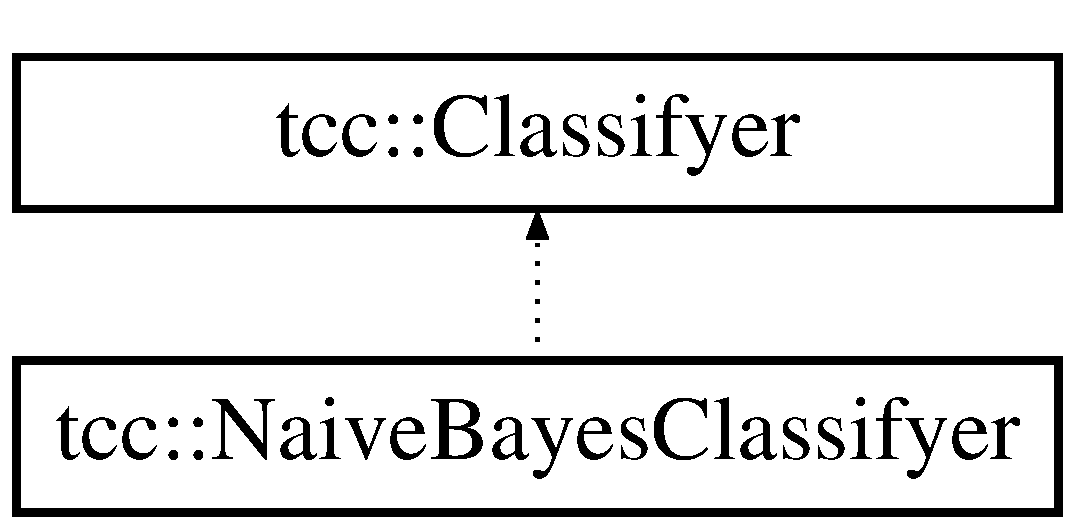
\includegraphics[height=2.000000cm]{classtcc_1_1_classifyer}
\end{center}
\end{figure}
\subsection*{Public Member Functions}
\begin{DoxyCompactItemize}
\item 
virtual void \hyperlink{classtcc_1_1_classifyer_a31a89d27c030b89964770d7ab5db7850}{train} ()=0\hypertarget{classtcc_1_1_classifyer_a31a89d27c030b89964770d7ab5db7850}{}\label{classtcc_1_1_classifyer_a31a89d27c030b89964770d7ab5db7850}

\begin{DoxyCompactList}\small\item\em Запуск обучения классификатора \end{DoxyCompactList}\item 
virtual double \hyperlink{classtcc_1_1_classifyer_a13db939fe0720f111df9266e1eef54c0}{run} (\hyperlink{namespacetcc_a9bdf9e81347b7904a6a7f8427d6465dc}{text\+Vec} \&\hyperlink{group__aliases_ga085c5ca5bf5645ff17c0ede30f56b08f}{text}) const  =0
\begin{DoxyCompactList}\small\item\em Оценка текста \end{DoxyCompactList}\end{DoxyCompactItemize}


\subsection{Detailed Description}
Интерфейс классификатора текста 

\subsection{Member Function Documentation}
\index{tcc\+::\+Classifyer@{tcc\+::\+Classifyer}!run@{run}}
\index{run@{run}!tcc\+::\+Classifyer@{tcc\+::\+Classifyer}}
\subsubsection[{\texorpdfstring{run(text\+Vec \&text) const  =0}{run(textVec &text) const  =0}}]{\setlength{\rightskip}{0pt plus 5cm}virtual double tcc\+::\+Classifyer\+::run (
\begin{DoxyParamCaption}
\item[{{\bf text\+Vec} \&}]{text}
\end{DoxyParamCaption}
) const\hspace{0.3cm}{\ttfamily [pure virtual]}}\hypertarget{classtcc_1_1_classifyer_a13db939fe0720f111df9266e1eef54c0}{}\label{classtcc_1_1_classifyer_a13db939fe0720f111df9266e1eef54c0}


Оценка текста 


\begin{DoxyParams}{Parameters}
{\em text} & -\/ текст, подлежащий оцениванию \\
\hline
\end{DoxyParams}
\begin{DoxyReturn}{Returns}
вероятность принадлежности текста категории 
\end{DoxyReturn}


Implemented in \hyperlink{classtcc_1_1_naive_bayes_classifyer_aec3d7dfdb8be9b48adf8e6489d97115d}{tcc\+::\+Naive\+Bayes\+Classifyer}.



The documentation for this class was generated from the following file\+:\begin{DoxyCompactItemize}
\item 
src/\+Classification/Classifyer.\+h\end{DoxyCompactItemize}

\hypertarget{classtcc_1_1_controller}{}\section{tcc\+:\+:Controller Class Reference}
\label{classtcc_1_1_controller}\index{tcc\+::\+Controller@{tcc\+::\+Controller}}


Основной класс контроллер управляющий ходом программы  




{\ttfamily \#include $<$Controller.\+h$>$}

\subsection*{Public Member Functions}
\begin{DoxyCompactItemize}
\item 
\hyperlink{classtcc_1_1_controller_addf3fea20133594d55a03f5134614b98}{Controller} (std\+::shared\+\_\+ptr$<$ \hyperlink{classtcc_1_1_data_provider}{Data\+Provider} $>$ data\+\_\+provider)
\begin{DoxyCompactList}\small\item\em Конструктор класса \end{DoxyCompactList}\item 
void \hyperlink{classtcc_1_1_controller_a61233522bd4c1a17dddb76f7f337bf3a}{init} ()\hypertarget{classtcc_1_1_controller_a61233522bd4c1a17dddb76f7f337bf3a}{}\label{classtcc_1_1_controller_a61233522bd4c1a17dddb76f7f337bf3a}

\begin{DoxyCompactList}\small\item\em Инициализация классификатора \end{DoxyCompactList}\item 
void \hyperlink{classtcc_1_1_controller_a41b047e081c2ae0350379b5d84e5d2a3}{run} (\hyperlink{namespacetcc_a9bdf9e81347b7904a6a7f8427d6465dc}{text\+Vec} \&texts)\hypertarget{classtcc_1_1_controller_a41b047e081c2ae0350379b5d84e5d2a3}{}\label{classtcc_1_1_controller_a41b047e081c2ae0350379b5d84e5d2a3}

\begin{DoxyCompactList}\small\item\em Обработка текста \end{DoxyCompactList}\item 
void \hyperlink{classtcc_1_1_controller_a957db61db1243fb15d8de927bfa90388}{save} ()\hypertarget{classtcc_1_1_controller_a957db61db1243fb15d8de927bfa90388}{}\label{classtcc_1_1_controller_a957db61db1243fb15d8de927bfa90388}

\begin{DoxyCompactList}\small\item\em Сохранить текущий результат \end{DoxyCompactList}\item 
void \hyperlink{classtcc_1_1_controller_a76359375dbebe6f184120f201c9b8821}{close} ()\hypertarget{classtcc_1_1_controller_a76359375dbebe6f184120f201c9b8821}{}\label{classtcc_1_1_controller_a76359375dbebe6f184120f201c9b8821}

\begin{DoxyCompactList}\small\item\em сохранить то, что осталось в буфере перед выыходом \end{DoxyCompactList}\end{DoxyCompactItemize}


\subsection{Detailed Description}
Основной класс контроллер управляющий ходом программы 

\subsection{Constructor \& Destructor Documentation}
\index{tcc\+::\+Controller@{tcc\+::\+Controller}!Controller@{Controller}}
\index{Controller@{Controller}!tcc\+::\+Controller@{tcc\+::\+Controller}}
\subsubsection[{\texorpdfstring{Controller(std\+::shared\+\_\+ptr$<$ Data\+Provider $>$ data\+\_\+provider)}{Controller(std::shared_ptr< DataProvider > data_provider)}}]{\setlength{\rightskip}{0pt plus 5cm}tcc\+::\+Controller\+::\+Controller (
\begin{DoxyParamCaption}
\item[{std\+::shared\+\_\+ptr$<$ {\bf Data\+Provider} $>$}]{data\+\_\+provider}
\end{DoxyParamCaption}
)\hspace{0.3cm}{\ttfamily [inline]}}\hypertarget{classtcc_1_1_controller_addf3fea20133594d55a03f5134614b98}{}\label{classtcc_1_1_controller_addf3fea20133594d55a03f5134614b98}


Конструктор класса 


\begin{DoxyParams}{Parameters}
{\em data\+\_\+provider} & Указатель на используемый провайдер \\
\hline
\end{DoxyParams}


The documentation for this class was generated from the following file\+:\begin{DoxyCompactItemize}
\item 
src/\+Controllers/Controller.\+h\end{DoxyCompactItemize}

\hypertarget{classtcc_1_1_core}{}\section{Класс tcc\+:\+:Core}
\label{classtcc_1_1_core}\index{tcc\+::\+Core@{tcc\+::\+Core}}


Интерфейс классов ядра для классификации \char`\"{}недоброжелательности\char`\"{} текста  




{\ttfamily \#include $<$Core.\+h$>$}

Граф наследования\+:tcc\+:\+:Core\+:\begin{figure}[H]
\begin{center}
\leavevmode
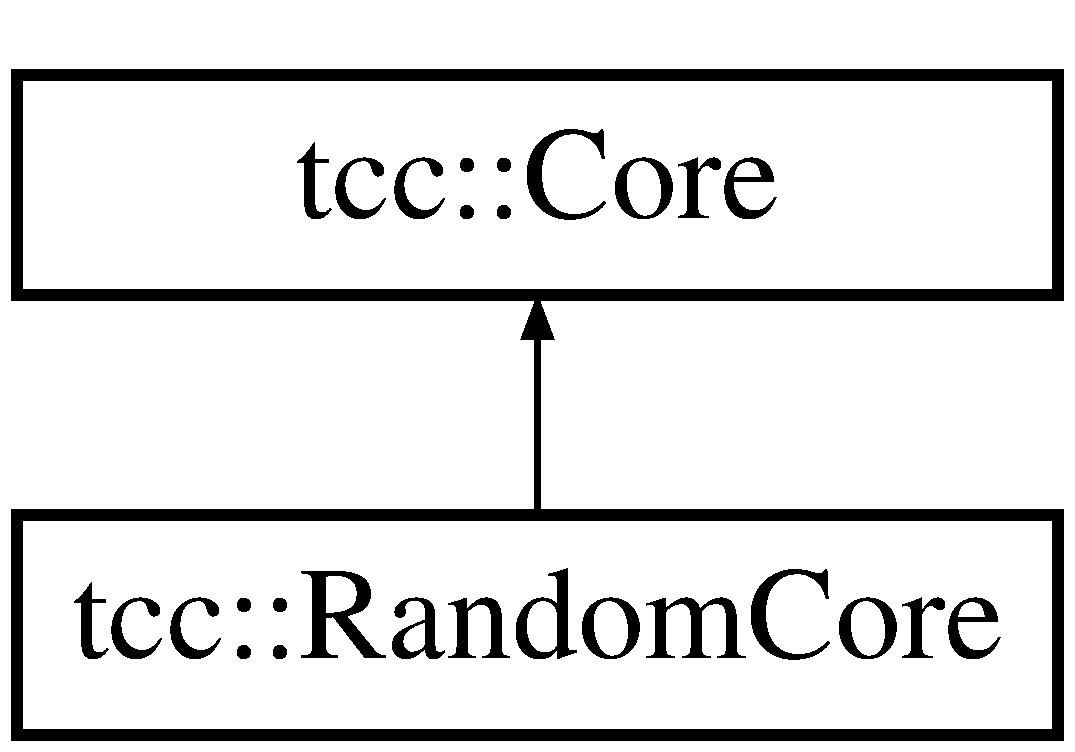
\includegraphics[height=2.000000cm]{classtcc_1_1_core}
\end{center}
\end{figure}


\subsection{Подробное описание}
Интерфейс классов ядра для классификации \char`\"{}недоброжелательности\char`\"{} текста 

См. определение в файле Core.\+h строка 14



Объявления и описания членов класса находятся в файле\+:\begin{DoxyCompactItemize}
\item 
Cores/Core.\+h\end{DoxyCompactItemize}

\hypertarget{classtcc_1_1_data_preprocessing}{}\section{tcc\+:\+:Data\+Preprocessing Class Reference}
\label{classtcc_1_1_data_preprocessing}\index{tcc\+::\+Data\+Preprocessing@{tcc\+::\+Data\+Preprocessing}}


Интерфейс для классов предобработки текста  




{\ttfamily \#include $<$Data\+Preprocessing.\+h$>$}



\subsection{Detailed Description}
Интерфейс для классов предобработки текста 

The documentation for this class was generated from the following file\+:\begin{DoxyCompactItemize}
\item 
src/\+Data\+Preprocessing/Data\+Preprocessing.\+h\end{DoxyCompactItemize}

\hypertarget{classtcc_1_1_data_provider}{}\section{tcc\+:\+:Data\+Provider Class Reference}
\label{classtcc_1_1_data_provider}\index{tcc\+::\+Data\+Provider@{tcc\+::\+Data\+Provider}}


Интерфейс для классов считывания/записи данных  




{\ttfamily \#include $<$Data\+Provider.\+h$>$}

Inheritance diagram for tcc\+:\+:Data\+Provider\+:\begin{figure}[H]
\begin{center}
\leavevmode
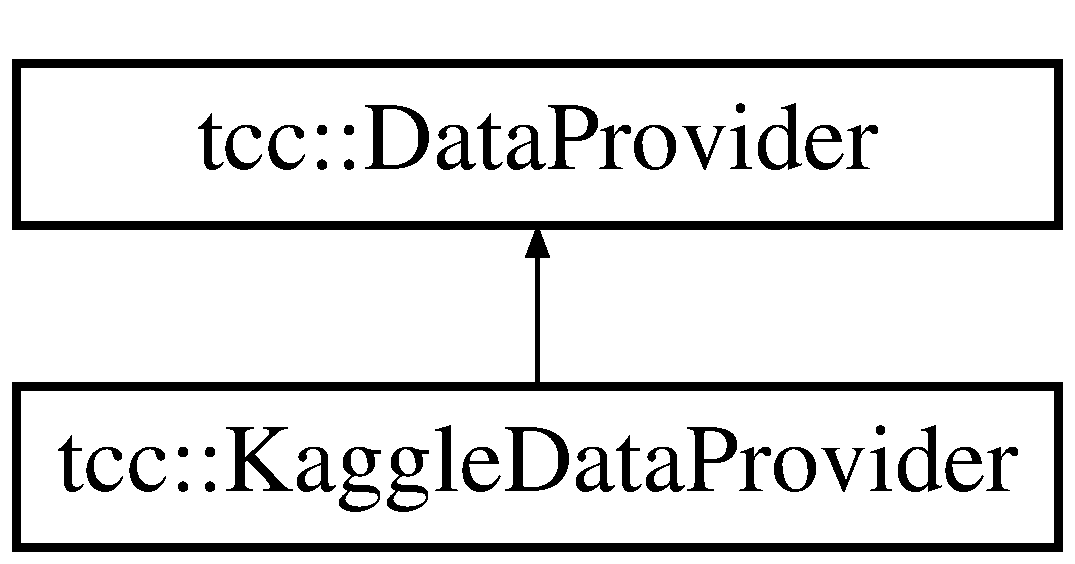
\includegraphics[height=2.000000cm]{classtcc_1_1_data_provider}
\end{center}
\end{figure}
\subsection*{Public Member Functions}
\begin{DoxyCompactItemize}
\item 
virtual std\+::vector$<$ json $>$ \hyperlink{classtcc_1_1_data_provider_af5a33d2b9d234e39547a148b8f99cf6f}{get\+\_\+data} () const  =0
\begin{DoxyCompactList}\small\item\em Виртуальная функция для считывания данных \end{DoxyCompactList}\end{DoxyCompactItemize}


\subsection{Detailed Description}
Интерфейс для классов считывания/записи данных 

\subsection{Member Function Documentation}
\index{tcc\+::\+Data\+Provider@{tcc\+::\+Data\+Provider}!get\+\_\+data@{get\+\_\+data}}
\index{get\+\_\+data@{get\+\_\+data}!tcc\+::\+Data\+Provider@{tcc\+::\+Data\+Provider}}
\subsubsection[{\texorpdfstring{get\+\_\+data() const  =0}{get_data() const  =0}}]{\setlength{\rightskip}{0pt plus 5cm}virtual std\+::vector$<$json$>$ tcc\+::\+Data\+Provider\+::get\+\_\+data (
\begin{DoxyParamCaption}
{}
\end{DoxyParamCaption}
) const\hspace{0.3cm}{\ttfamily [pure virtual]}}\hypertarget{classtcc_1_1_data_provider_af5a33d2b9d234e39547a148b8f99cf6f}{}\label{classtcc_1_1_data_provider_af5a33d2b9d234e39547a148b8f99cf6f}


Виртуальная функция для считывания данных 

\begin{DoxyReturn}{Returns}
Вектор структур данных, содержащих в себе считанные данные 
\end{DoxyReturn}

\begin{DoxyExceptions}{Exceptions}
{\em I\+O\+Exception} & Исключение возникающее при проблемах с чтением файла \\
\hline
\end{DoxyExceptions}


Implemented in \hyperlink{classtcc_1_1_kaggle_data_provider_a9a70415967019e9199957bf208a31478}{tcc\+::\+Kaggle\+Data\+Provider}.



The documentation for this class was generated from the following file\+:\begin{DoxyCompactItemize}
\item 
src/\+Data\+Providers/Data\+Provider.\+h\end{DoxyCompactItemize}

\hypertarget{classtcc_1_1_features}{}\section{tcc\+:\+:Features Class Reference}
\label{classtcc_1_1_features}\index{tcc\+::\+Features@{tcc\+::\+Features}}


Интерфейс класса, преобразующего текст в вектор  




{\ttfamily \#include $<$Vocab.\+h$>$}

Inheritance diagram for tcc\+:\+:Features\+:\begin{figure}[H]
\begin{center}
\leavevmode
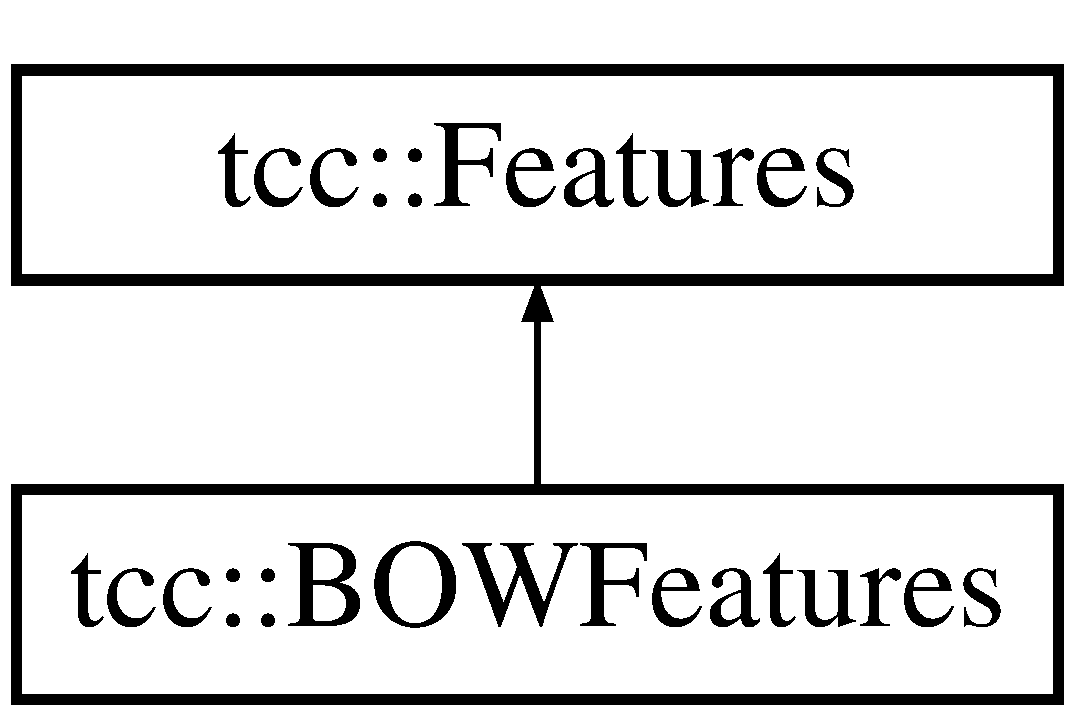
\includegraphics[height=2.000000cm]{classtcc_1_1_features}
\end{center}
\end{figure}
\subsection*{Public Member Functions}
\begin{DoxyCompactItemize}
\item 
virtual \hyperlink{group__aliases_gae00908f082db728f73e52c3b4932261a}{uint} \hyperlink{classtcc_1_1_features_a840094cf14bfb563d7820e39ae8c6d48}{extract\+\_\+feature} (std\+::string \&s, std\+::function$<$ double(double)$>$ f) const  =0
\begin{DoxyCompactList}\small\item\em Оценка выраженности признака, задаваемого одним словом \end{DoxyCompactList}\item 
virtual \hyperlink{group__aliases_gae00908f082db728f73e52c3b4932261a}{uint} \hyperlink{classtcc_1_1_features_ad70d9deac212689322d4d4e88cff26e3}{extract\+\_\+feature} (\hyperlink{group__aliases_ga085c5ca5bf5645ff17c0ede30f56b08f}{text} \&s, std\+::function$<$ double(double)$>$ f) const  =0
\begin{DoxyCompactList}\small\item\em Оценка выраженности признака, задаваемого несколькими словами \end{DoxyCompactList}\item 
virtual \hyperlink{group__aliases_gae00908f082db728f73e52c3b4932261a}{uint} \hyperlink{classtcc_1_1_features_ae87452022b079681e9904efd4ffbe201}{reduce\+\_\+dimensions} (\hyperlink{group__aliases_gae00908f082db728f73e52c3b4932261a}{uint} dim, \hyperlink{group__aliases_ga085c5ca5bf5645ff17c0ede30f56b08f}{text} \&s, std\+::function$<$ double(double)$>$ f) const  =0
\begin{DoxyCompactList}\small\item\em Сжатие размерности \end{DoxyCompactList}\item 
double \hyperlink{classtcc_1_1_features_af03f2694924c4522c70d41a4a6503ff0}{metric} (\hyperlink{classtcc_1_1_features}{Features} \&l, \hyperlink{classtcc_1_1_features}{Features} \&r)
\begin{DoxyCompactList}\small\item\em Оценка расстояния между двумя текстами \end{DoxyCompactList}\end{DoxyCompactItemize}


\subsection{Detailed Description}
Интерфейс класса, преобразующего текст в вектор 

\subsection{Member Function Documentation}
\index{tcc\+::\+Features@{tcc\+::\+Features}!extract\+\_\+feature@{extract\+\_\+feature}}
\index{extract\+\_\+feature@{extract\+\_\+feature}!tcc\+::\+Features@{tcc\+::\+Features}}
\subsubsection[{\texorpdfstring{extract\+\_\+feature(std\+::string \&s, std\+::function$<$ double(double)$>$ f) const  =0}{extract_feature(std::string &s, std::function< double(double)> f) const  =0}}]{\setlength{\rightskip}{0pt plus 5cm}virtual {\bf uint} tcc\+::\+Features\+::extract\+\_\+feature (
\begin{DoxyParamCaption}
\item[{std\+::string \&}]{s, }
\item[{std\+::function$<$ double(double)$>$}]{f}
\end{DoxyParamCaption}
) const\hspace{0.3cm}{\ttfamily [pure virtual]}}\hypertarget{classtcc_1_1_features_a840094cf14bfb563d7820e39ae8c6d48}{}\label{classtcc_1_1_features_a840094cf14bfb563d7820e39ae8c6d48}


Оценка выраженности признака, задаваемого одним словом 


\begin{DoxyParams}{Parameters}
{\em s} & текст \\
\hline
{\em f} & функция, с помощью которой оценивается выраженность признака \\
\hline
\end{DoxyParams}
\index{tcc\+::\+Features@{tcc\+::\+Features}!extract\+\_\+feature@{extract\+\_\+feature}}
\index{extract\+\_\+feature@{extract\+\_\+feature}!tcc\+::\+Features@{tcc\+::\+Features}}
\subsubsection[{\texorpdfstring{extract\+\_\+feature(text \&s, std\+::function$<$ double(double)$>$ f) const  =0}{extract_feature(text &s, std::function< double(double)> f) const  =0}}]{\setlength{\rightskip}{0pt plus 5cm}virtual {\bf uint} tcc\+::\+Features\+::extract\+\_\+feature (
\begin{DoxyParamCaption}
\item[{{\bf text} \&}]{s, }
\item[{std\+::function$<$ double(double)$>$}]{f}
\end{DoxyParamCaption}
) const\hspace{0.3cm}{\ttfamily [pure virtual]}}\hypertarget{classtcc_1_1_features_ad70d9deac212689322d4d4e88cff26e3}{}\label{classtcc_1_1_features_ad70d9deac212689322d4d4e88cff26e3}


Оценка выраженности признака, задаваемого несколькими словами 


\begin{DoxyParams}{Parameters}
{\em s} & текст \\
\hline
{\em f} & функция, с помощью которой оценивается выраженность признака \\
\hline
\end{DoxyParams}
\index{tcc\+::\+Features@{tcc\+::\+Features}!metric@{metric}}
\index{metric@{metric}!tcc\+::\+Features@{tcc\+::\+Features}}
\subsubsection[{\texorpdfstring{metric(\+Features \&l, Features \&r)}{metric(Features &l, Features &r)}}]{\setlength{\rightskip}{0pt plus 5cm}double tcc\+::\+Features\+::metric (
\begin{DoxyParamCaption}
\item[{{\bf Features} \&}]{l, }
\item[{{\bf Features} \&}]{r}
\end{DoxyParamCaption}
)}\hypertarget{classtcc_1_1_features_af03f2694924c4522c70d41a4a6503ff0}{}\label{classtcc_1_1_features_af03f2694924c4522c70d41a4a6503ff0}


Оценка расстояния между двумя текстами 


\begin{DoxyParams}{Parameters}
{\em l,r} & тексты \\
\hline
\end{DoxyParams}
\index{tcc\+::\+Features@{tcc\+::\+Features}!reduce\+\_\+dimensions@{reduce\+\_\+dimensions}}
\index{reduce\+\_\+dimensions@{reduce\+\_\+dimensions}!tcc\+::\+Features@{tcc\+::\+Features}}
\subsubsection[{\texorpdfstring{reduce\+\_\+dimensions(uint dim, text \&s, std\+::function$<$ double(double)$>$ f) const  =0}{reduce_dimensions(uint dim, text &s, std::function< double(double)> f) const  =0}}]{\setlength{\rightskip}{0pt plus 5cm}virtual {\bf uint} tcc\+::\+Features\+::reduce\+\_\+dimensions (
\begin{DoxyParamCaption}
\item[{{\bf uint}}]{dim, }
\item[{{\bf text} \&}]{s, }
\item[{std\+::function$<$ double(double)$>$}]{f}
\end{DoxyParamCaption}
) const\hspace{0.3cm}{\ttfamily [pure virtual]}}\hypertarget{classtcc_1_1_features_ae87452022b079681e9904efd4ffbe201}{}\label{classtcc_1_1_features_ae87452022b079681e9904efd4ffbe201}


Сжатие размерности 


\begin{DoxyParams}{Parameters}
{\em dim} & желаемая размерность \\
\hline
{\em s} & текст \\
\hline
{\em f} & функция, с помощью которой производится сжатие \\
\hline
\end{DoxyParams}


The documentation for this class was generated from the following file\+:\begin{DoxyCompactItemize}
\item 
src/\+Classification/Vocab.\+h\end{DoxyCompactItemize}

\hypertarget{class_g_u_i_main_window}{}\section{G\+U\+I\+Main\+Window Class Reference}
\label{class_g_u_i_main_window}\index{G\+U\+I\+Main\+Window@{G\+U\+I\+Main\+Window}}


Qt окно  




{\ttfamily \#include $<$mainwindow.\+h$>$}

Inheritance diagram for G\+U\+I\+Main\+Window\+:\begin{figure}[H]
\begin{center}
\leavevmode
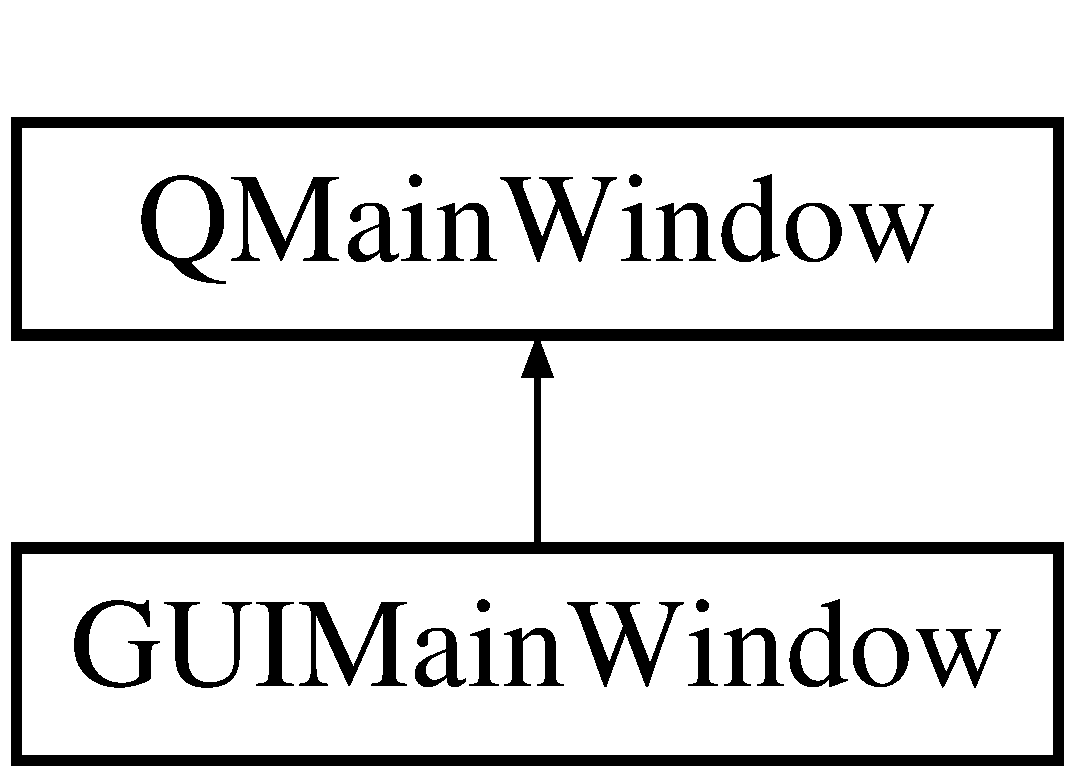
\includegraphics[height=2.000000cm]{class_g_u_i_main_window}
\end{center}
\end{figure}
\subsection*{Public Member Functions}
\begin{DoxyCompactItemize}
\item 
\hyperlink{class_g_u_i_main_window_a15dd59ceaf094244961e4b66a5aa890a}{G\+U\+I\+Main\+Window} (Q\+Widget $\ast$parent=0)
\begin{DoxyCompactList}\small\item\em Конструктор класса. \end{DoxyCompactList}\item 
\hyperlink{class_g_u_i_main_window_a16ca27363f15a5f2678417bbf26880d2}{$\sim$\+G\+U\+I\+Main\+Window} ()\hypertarget{class_g_u_i_main_window_a16ca27363f15a5f2678417bbf26880d2}{}\label{class_g_u_i_main_window_a16ca27363f15a5f2678417bbf26880d2}

\begin{DoxyCompactList}\small\item\em Деструктор класса. \end{DoxyCompactList}\end{DoxyCompactItemize}


\subsection{Detailed Description}
Qt окно 

\subsection{Constructor \& Destructor Documentation}
\index{G\+U\+I\+Main\+Window@{G\+U\+I\+Main\+Window}!G\+U\+I\+Main\+Window@{G\+U\+I\+Main\+Window}}
\index{G\+U\+I\+Main\+Window@{G\+U\+I\+Main\+Window}!G\+U\+I\+Main\+Window@{G\+U\+I\+Main\+Window}}
\subsubsection[{\texorpdfstring{G\+U\+I\+Main\+Window(\+Q\+Widget $\ast$parent=0)}{GUIMainWindow(QWidget *parent=0)}}]{\setlength{\rightskip}{0pt plus 5cm}G\+U\+I\+Main\+Window\+::\+G\+U\+I\+Main\+Window (
\begin{DoxyParamCaption}
\item[{Q\+Widget $\ast$}]{parent = {\ttfamily 0}}
\end{DoxyParamCaption}
)\hspace{0.3cm}{\ttfamily [explicit]}}\hypertarget{class_g_u_i_main_window_a15dd59ceaf094244961e4b66a5aa890a}{}\label{class_g_u_i_main_window_a15dd59ceaf094244961e4b66a5aa890a}


Конструктор класса. 


\begin{DoxyParams}{Parameters}
{\em parent} & Родительский виджет. \\
\hline
\end{DoxyParams}


The documentation for this class was generated from the following file\+:\begin{DoxyCompactItemize}
\item 
src/\+G\+U\+I/mainwindow.\+h\end{DoxyCompactItemize}

\hypertarget{classtcc_1_1_kaggle_data_provider}{}\section{tcc\+:\+:Kaggle\+Data\+Provider Class Reference}
\label{classtcc_1_1_kaggle_data_provider}\index{tcc\+::\+Kaggle\+Data\+Provider@{tcc\+::\+Kaggle\+Data\+Provider}}


Класс для считывания тренировочных образцов с сайта Kaggle.  




{\ttfamily \#include $<$Data\+Provider.\+h$>$}

Inheritance diagram for tcc\+:\+:Kaggle\+Data\+Provider\+:\begin{figure}[H]
\begin{center}
\leavevmode
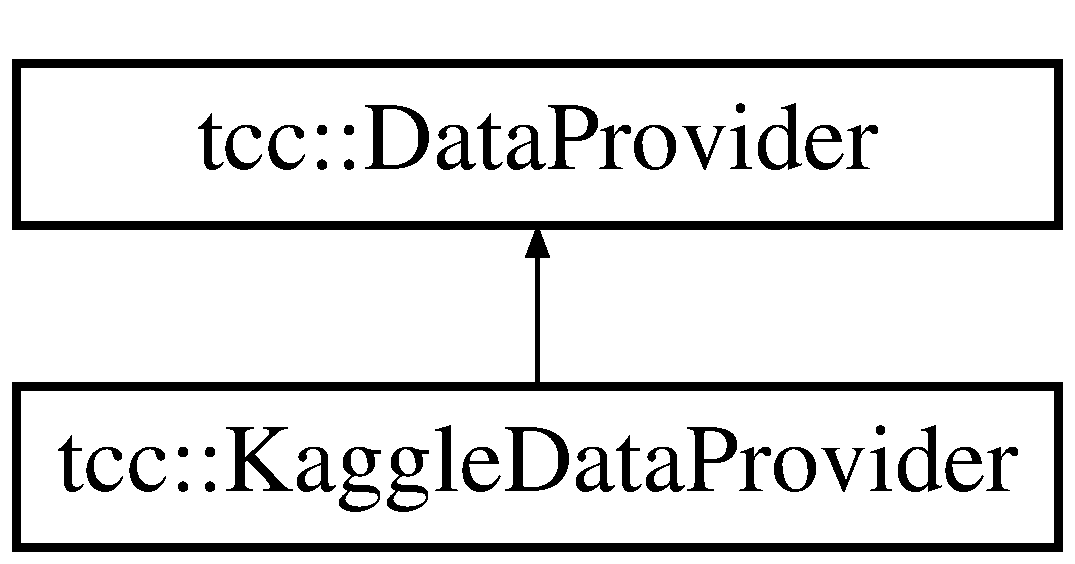
\includegraphics[height=2.000000cm]{classtcc_1_1_kaggle_data_provider}
\end{center}
\end{figure}
\subsection*{Public Member Functions}
\begin{DoxyCompactItemize}
\item 
\hyperlink{classtcc_1_1_kaggle_data_provider_aac9b42f0803107edf1b3d66cc143f862}{Kaggle\+Data\+Provider} (std\+::string \&input\+\_\+file)
\begin{DoxyCompactList}\small\item\em Конструктор класса \end{DoxyCompactList}\item 
\hyperlink{classtcc_1_1_kaggle_data_provider_af650fc5c99e7fd507f48ec057fd34d21}{Kaggle\+Data\+Provider} (const \hyperlink{classtcc_1_1_kaggle_data_provider}{Kaggle\+Data\+Provider} \&rv)
\begin{DoxyCompactList}\small\item\em Конструктор копии экземпляра класса \end{DoxyCompactList}\item 
std\+::vector$<$ json $>$ \hyperlink{classtcc_1_1_kaggle_data_provider_a9a70415967019e9199957bf208a31478}{get\+\_\+data} () const  override
\begin{DoxyCompactList}\small\item\em Функция для считывания данных из файла \end{DoxyCompactList}\end{DoxyCompactItemize}


\subsection{Detailed Description}
Класс для считывания тренировочных образцов с сайта Kaggle. 

\subsection{Constructor \& Destructor Documentation}
\index{tcc\+::\+Kaggle\+Data\+Provider@{tcc\+::\+Kaggle\+Data\+Provider}!Kaggle\+Data\+Provider@{Kaggle\+Data\+Provider}}
\index{Kaggle\+Data\+Provider@{Kaggle\+Data\+Provider}!tcc\+::\+Kaggle\+Data\+Provider@{tcc\+::\+Kaggle\+Data\+Provider}}
\subsubsection[{\texorpdfstring{Kaggle\+Data\+Provider(std\+::string \&input\+\_\+file)}{KaggleDataProvider(std::string &input_file)}}]{\setlength{\rightskip}{0pt plus 5cm}tcc\+::\+Kaggle\+Data\+Provider\+::\+Kaggle\+Data\+Provider (
\begin{DoxyParamCaption}
\item[{std\+::string \&}]{input\+\_\+file}
\end{DoxyParamCaption}
)\hspace{0.3cm}{\ttfamily [inline]}}\hypertarget{classtcc_1_1_kaggle_data_provider_aac9b42f0803107edf1b3d66cc143f862}{}\label{classtcc_1_1_kaggle_data_provider_aac9b42f0803107edf1b3d66cc143f862}


Конструктор класса 


\begin{DoxyParams}{Parameters}
{\em input\+\_\+file} & Имя файла для чтения \\
\hline
\end{DoxyParams}
\index{tcc\+::\+Kaggle\+Data\+Provider@{tcc\+::\+Kaggle\+Data\+Provider}!Kaggle\+Data\+Provider@{Kaggle\+Data\+Provider}}
\index{Kaggle\+Data\+Provider@{Kaggle\+Data\+Provider}!tcc\+::\+Kaggle\+Data\+Provider@{tcc\+::\+Kaggle\+Data\+Provider}}
\subsubsection[{\texorpdfstring{Kaggle\+Data\+Provider(const Kaggle\+Data\+Provider \&rv)}{KaggleDataProvider(const KaggleDataProvider &rv)}}]{\setlength{\rightskip}{0pt plus 5cm}tcc\+::\+Kaggle\+Data\+Provider\+::\+Kaggle\+Data\+Provider (
\begin{DoxyParamCaption}
\item[{const {\bf Kaggle\+Data\+Provider} \&}]{rv}
\end{DoxyParamCaption}
)\hspace{0.3cm}{\ttfamily [inline]}}\hypertarget{classtcc_1_1_kaggle_data_provider_af650fc5c99e7fd507f48ec057fd34d21}{}\label{classtcc_1_1_kaggle_data_provider_af650fc5c99e7fd507f48ec057fd34d21}


Конструктор копии экземпляра класса 


\begin{DoxyParams}{Parameters}
{\em rv} & Копируемый экземпляр \\
\hline
\end{DoxyParams}


\subsection{Member Function Documentation}
\index{tcc\+::\+Kaggle\+Data\+Provider@{tcc\+::\+Kaggle\+Data\+Provider}!get\+\_\+data@{get\+\_\+data}}
\index{get\+\_\+data@{get\+\_\+data}!tcc\+::\+Kaggle\+Data\+Provider@{tcc\+::\+Kaggle\+Data\+Provider}}
\subsubsection[{\texorpdfstring{get\+\_\+data() const  override}{get_data() const  override}}]{\setlength{\rightskip}{0pt plus 5cm}std\+::vector$<$json$>$ tcc\+::\+Kaggle\+Data\+Provider\+::get\+\_\+data (
\begin{DoxyParamCaption}
{}
\end{DoxyParamCaption}
) const\hspace{0.3cm}{\ttfamily [override]}, {\ttfamily [virtual]}}\hypertarget{classtcc_1_1_kaggle_data_provider_a9a70415967019e9199957bf208a31478}{}\label{classtcc_1_1_kaggle_data_provider_a9a70415967019e9199957bf208a31478}


Функция для считывания данных из файла 

\begin{DoxyReturn}{Returns}
Вектор структур данных, содержащих в себе считанные данные 
\end{DoxyReturn}

\begin{DoxyExceptions}{Exceptions}
{\em I\+O\+Exception} & Исключение возникающее при проблемах с чтением файла \\
\hline
\end{DoxyExceptions}


Implements \hyperlink{classtcc_1_1_data_provider_af5a33d2b9d234e39547a148b8f99cf6f}{tcc\+::\+Data\+Provider}.



The documentation for this class was generated from the following file\+:\begin{DoxyCompactItemize}
\item 
src/\+Data\+Providers/Data\+Provider.\+h\end{DoxyCompactItemize}

\hypertarget{classtcc_1_1_naive_bayes_classifyer}{}\section{tcc\+:\+:Naive\+Bayes\+Classifyer Class Reference}
\label{classtcc_1_1_naive_bayes_classifyer}\index{tcc\+::\+Naive\+Bayes\+Classifyer@{tcc\+::\+Naive\+Bayes\+Classifyer}}


Наивный байесовский классификатор  




{\ttfamily \#include $<$Classifyer.\+h$>$}

Inheritance diagram for tcc\+:\+:Naive\+Bayes\+Classifyer\+:\begin{figure}[H]
\begin{center}
\leavevmode
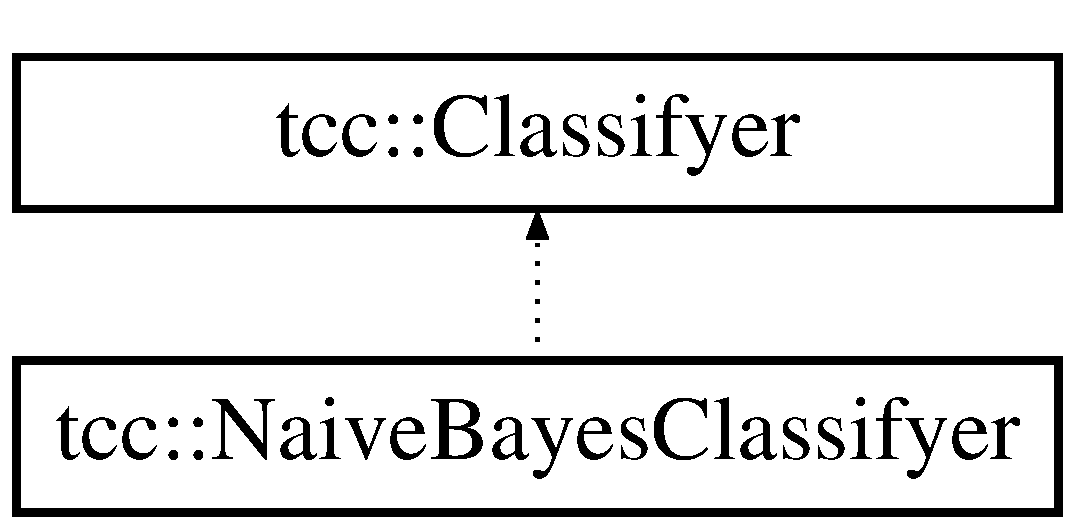
\includegraphics[height=2.000000cm]{classtcc_1_1_naive_bayes_classifyer}
\end{center}
\end{figure}
\subsection*{Public Member Functions}
\begin{DoxyCompactItemize}
\item 
\hyperlink{classtcc_1_1_naive_bayes_classifyer_ae49c42da81a9dd855bd09b2cb4f6816c}{Naive\+Bayes\+Classifyer} (std\+::shared\+\_\+ptr$<$ \hyperlink{classtcc_1_1_features}{Features} $>$ \&v)
\begin{DoxyCompactList}\small\item\em Конструктор экземпляра класса \end{DoxyCompactList}\item 
void \hyperlink{classtcc_1_1_naive_bayes_classifyer_a2e33142e454481ff8d217626050c54a7}{train} () override\hypertarget{classtcc_1_1_naive_bayes_classifyer_a2e33142e454481ff8d217626050c54a7}{}\label{classtcc_1_1_naive_bayes_classifyer_a2e33142e454481ff8d217626050c54a7}

\begin{DoxyCompactList}\small\item\em Запуск обучения классификатора \end{DoxyCompactList}\item 
double \hyperlink{classtcc_1_1_naive_bayes_classifyer_aec3d7dfdb8be9b48adf8e6489d97115d}{run} (\hyperlink{namespacetcc_a9bdf9e81347b7904a6a7f8427d6465dc}{text\+Vec} \&\hyperlink{group__aliases_ga085c5ca5bf5645ff17c0ede30f56b08f}{text}) const  override
\begin{DoxyCompactList}\small\item\em Оценка текста \end{DoxyCompactList}\end{DoxyCompactItemize}


\subsection{Detailed Description}
Наивный байесовский классификатор 

\subsection{Constructor \& Destructor Documentation}
\index{tcc\+::\+Naive\+Bayes\+Classifyer@{tcc\+::\+Naive\+Bayes\+Classifyer}!Naive\+Bayes\+Classifyer@{Naive\+Bayes\+Classifyer}}
\index{Naive\+Bayes\+Classifyer@{Naive\+Bayes\+Classifyer}!tcc\+::\+Naive\+Bayes\+Classifyer@{tcc\+::\+Naive\+Bayes\+Classifyer}}
\subsubsection[{\texorpdfstring{Naive\+Bayes\+Classifyer(std\+::shared\+\_\+ptr$<$ Features $>$ \&v)}{NaiveBayesClassifyer(std::shared_ptr< Features > &v)}}]{\setlength{\rightskip}{0pt plus 5cm}tcc\+::\+Naive\+Bayes\+Classifyer\+::\+Naive\+Bayes\+Classifyer (
\begin{DoxyParamCaption}
\item[{std\+::shared\+\_\+ptr$<$ {\bf Features} $>$ \&}]{v}
\end{DoxyParamCaption}
)\hspace{0.3cm}{\ttfamily [inline]}}\hypertarget{classtcc_1_1_naive_bayes_classifyer_ae49c42da81a9dd855bd09b2cb4f6816c}{}\label{classtcc_1_1_naive_bayes_classifyer_ae49c42da81a9dd855bd09b2cb4f6816c}


Конструктор экземпляра класса 


\begin{DoxyParams}{Parameters}
{\em v} & -\/ информация о словах, встречающихся в корпусе текстов \\
\hline
\end{DoxyParams}


\subsection{Member Function Documentation}
\index{tcc\+::\+Naive\+Bayes\+Classifyer@{tcc\+::\+Naive\+Bayes\+Classifyer}!run@{run}}
\index{run@{run}!tcc\+::\+Naive\+Bayes\+Classifyer@{tcc\+::\+Naive\+Bayes\+Classifyer}}
\subsubsection[{\texorpdfstring{run(text\+Vec \&text) const  override}{run(textVec &text) const  override}}]{\setlength{\rightskip}{0pt plus 5cm}double tcc\+::\+Naive\+Bayes\+Classifyer\+::run (
\begin{DoxyParamCaption}
\item[{{\bf text\+Vec} \&}]{text}
\end{DoxyParamCaption}
) const\hspace{0.3cm}{\ttfamily [override]}, {\ttfamily [virtual]}}\hypertarget{classtcc_1_1_naive_bayes_classifyer_aec3d7dfdb8be9b48adf8e6489d97115d}{}\label{classtcc_1_1_naive_bayes_classifyer_aec3d7dfdb8be9b48adf8e6489d97115d}


Оценка текста 


\begin{DoxyParams}{Parameters}
{\em text} & -\/ текст, подлежащий оцениванию \\
\hline
\end{DoxyParams}
\begin{DoxyReturn}{Returns}
вероятность принадлежности текста категории 
\end{DoxyReturn}


Implements \hyperlink{classtcc_1_1_classifyer_a13db939fe0720f111df9266e1eef54c0}{tcc\+::\+Classifyer}.



The documentation for this class was generated from the following file\+:\begin{DoxyCompactItemize}
\item 
src/\+Classification/Classifyer.\+h\end{DoxyCompactItemize}

\hypertarget{classtcc_1_1_porter_stemming}{}\section{tcc\+:\+:Porter\+Stemming Class Reference}
\label{classtcc_1_1_porter_stemming}\index{tcc\+::\+Porter\+Stemming@{tcc\+::\+Porter\+Stemming}}


Стеммер Портера  




{\ttfamily \#include $<$Stemmer.\+h$>$}

Inheritance diagram for tcc\+:\+:Porter\+Stemming\+:\begin{figure}[H]
\begin{center}
\leavevmode
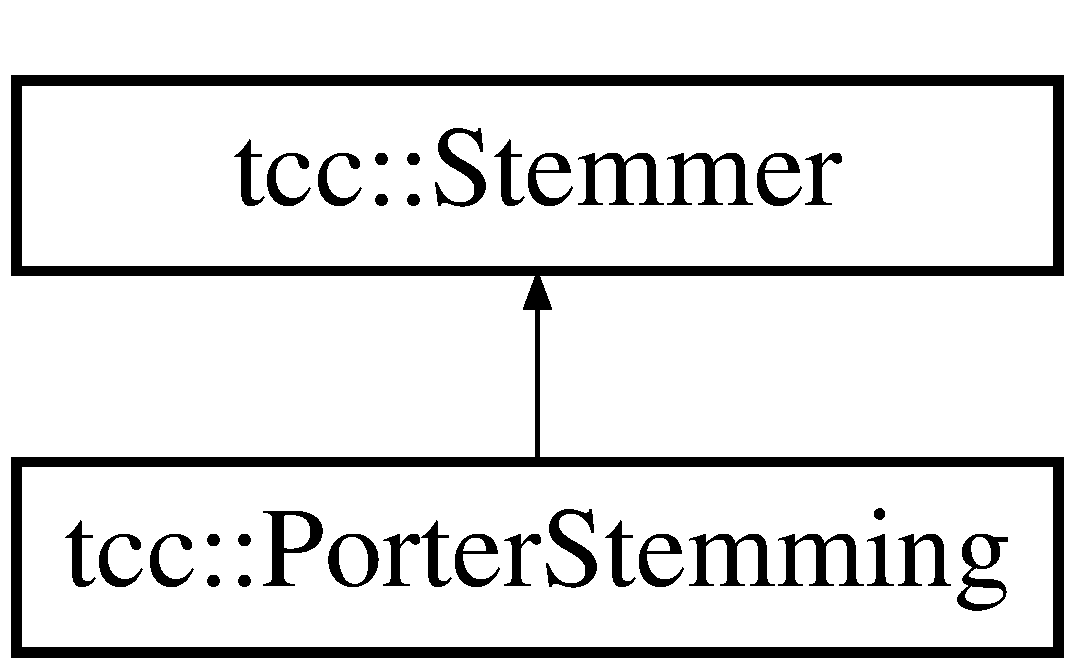
\includegraphics[height=2.000000cm]{classtcc_1_1_porter_stemming}
\end{center}
\end{figure}
\subsection*{Public Member Functions}
\begin{DoxyCompactItemize}
\item 
std\+::vector$<$ std\+::vector$<$ \hyperlink{namespacetcc_a310a95f44f9f0b3198b9758732eba6b9}{tcc\+::word\+\_\+t} $>$ $>$ \hyperlink{classtcc_1_1_porter_stemming_a55589afcaad97b491ec344cc24a889d9}{stem} (std\+::vector$<$ json $>$ \hyperlink{group__aliases_ga085c5ca5bf5645ff17c0ede30f56b08f}{text})
\begin{DoxyCompactList}\small\item\em Функция, реализующая Стеммер Портера \end{DoxyCompactList}\end{DoxyCompactItemize}


\subsection{Detailed Description}
Стеммер Портера 

\subsection{Member Function Documentation}
\index{tcc\+::\+Porter\+Stemming@{tcc\+::\+Porter\+Stemming}!stem@{stem}}
\index{stem@{stem}!tcc\+::\+Porter\+Stemming@{tcc\+::\+Porter\+Stemming}}
\subsubsection[{\texorpdfstring{stem(std\+::vector$<$ json $>$ text)}{stem(std::vector< json > text)}}]{\setlength{\rightskip}{0pt plus 5cm}std\+::vector$<$std\+::vector$<${\bf tcc\+::word\+\_\+t}$>$ $>$ tcc\+::\+Porter\+Stemming\+::stem (
\begin{DoxyParamCaption}
\item[{std\+::vector$<$ json $>$}]{text}
\end{DoxyParamCaption}
)\hspace{0.3cm}{\ttfamily [virtual]}}\hypertarget{classtcc_1_1_porter_stemming_a55589afcaad97b491ec344cc24a889d9}{}\label{classtcc_1_1_porter_stemming_a55589afcaad97b491ec344cc24a889d9}


Функция, реализующая Стеммер Портера 


\begin{DoxyParams}{Parameters}
{\em text} & Структура данных, содержащая в себе текст, подлежащий стеммингу \\
\hline
\end{DoxyParams}
\begin{DoxyReturn}{Returns}
Структура данных, содержащая в себе слова, приведенные к начальной форме 
\end{DoxyReturn}


Implements \hyperlink{classtcc_1_1_stemmer_a0131d8cb63b514e594d2407048687cff}{tcc\+::\+Stemmer}.



The documentation for this class was generated from the following file\+:\begin{DoxyCompactItemize}
\item 
src/\+Stemmer/Stemmer.\+h\end{DoxyCompactItemize}

\hypertarget{classtcc_1_1_random_core}{}\section{Класс tcc\+:\+:Random\+Core}
\label{classtcc_1_1_random_core}\index{tcc\+::\+Random\+Core@{tcc\+::\+Random\+Core}}


Класс -\/ ядро для классификации \char`\"{}недоброжелательности\char`\"{} текста  




{\ttfamily \#include $<$Core.\+h$>$}

Граф наследования\+:tcc\+:\+:Random\+Core\+:\begin{figure}[H]
\begin{center}
\leavevmode
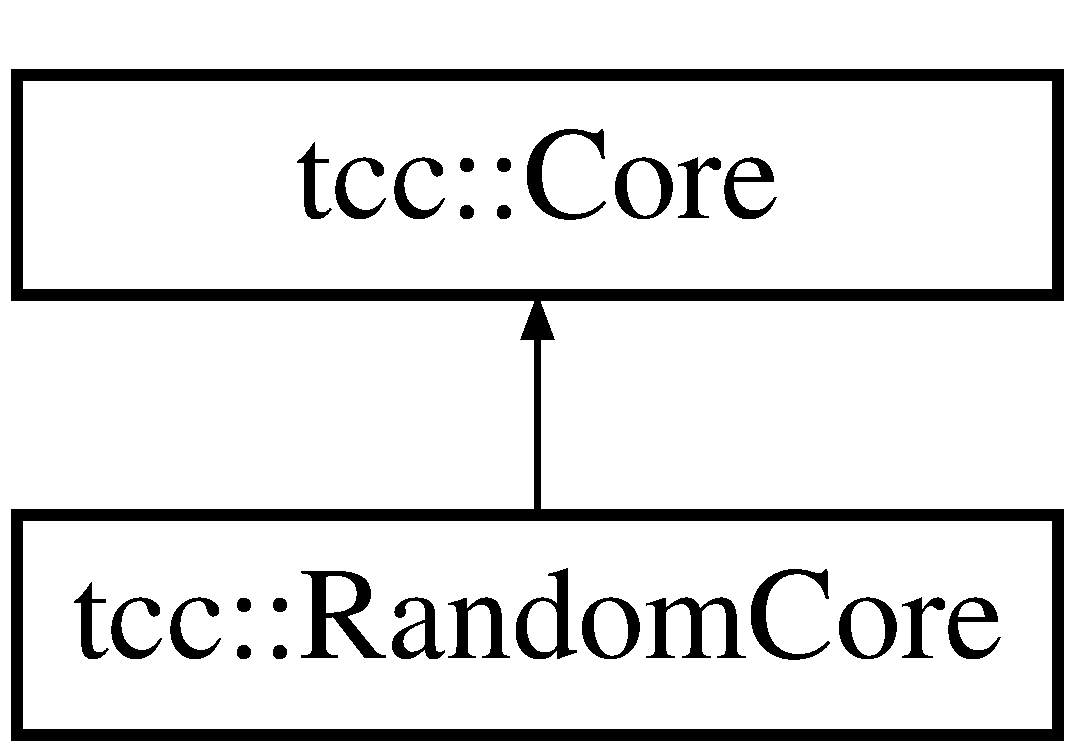
\includegraphics[height=2.000000cm]{classtcc_1_1_random_core}
\end{center}
\end{figure}


\subsection{Подробное описание}
Класс -\/ ядро для классификации \char`\"{}недоброжелательности\char`\"{} текста 

См. определение в файле Core.\+h строка 25



Объявления и описания членов класса находятся в файле\+:\begin{DoxyCompactItemize}
\item 
Cores/Core.\+h\end{DoxyCompactItemize}

\hypertarget{classtcc_1_1_stemmer}{}\section{tcc\+:\+:Stemmer Class Reference}
\label{classtcc_1_1_stemmer}\index{tcc\+::\+Stemmer@{tcc\+::\+Stemmer}}


Интерфейс для классов, предназначенных для нахождения основы слова (стемминга)  




{\ttfamily \#include $<$Stemmer.\+h$>$}

Inheritance diagram for tcc\+:\+:Stemmer\+:\begin{figure}[H]
\begin{center}
\leavevmode
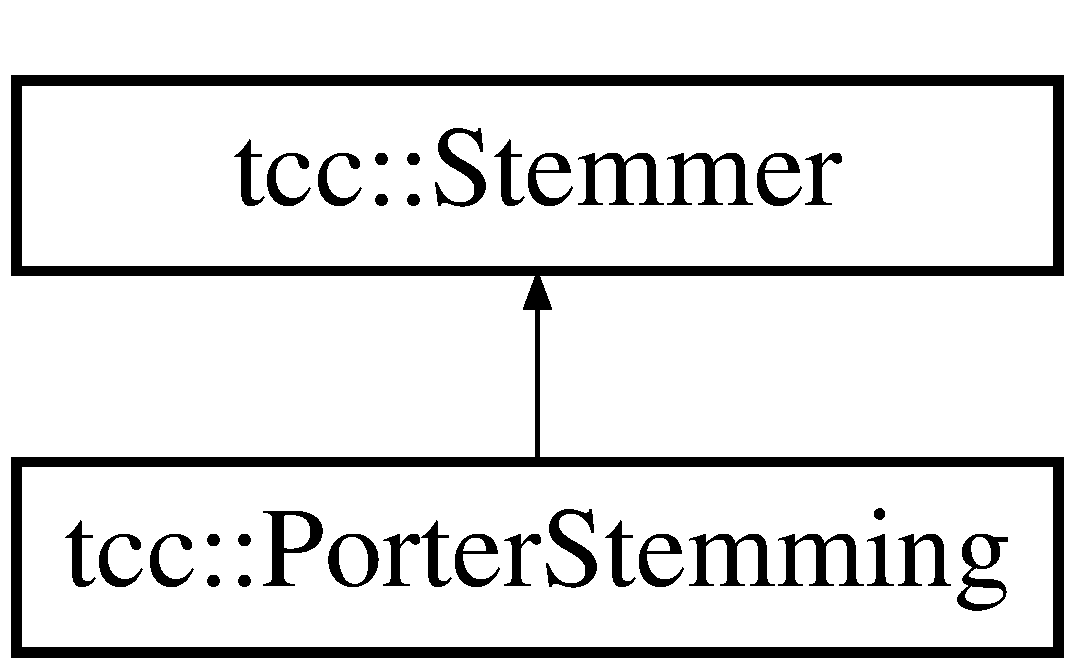
\includegraphics[height=2.000000cm]{classtcc_1_1_stemmer}
\end{center}
\end{figure}
\subsection*{Public Member Functions}
\begin{DoxyCompactItemize}
\item 
virtual std\+::vector$<$ std\+::vector$<$ \hyperlink{namespacetcc_a310a95f44f9f0b3198b9758732eba6b9}{tcc\+::word\+\_\+t} $>$ $>$ \hyperlink{classtcc_1_1_stemmer_a0131d8cb63b514e594d2407048687cff}{stem} (std\+::vector$<$ json $>$ \hyperlink{group__aliases_ga085c5ca5bf5645ff17c0ede30f56b08f}{text})=0
\begin{DoxyCompactList}\small\item\em Виртуальная функция для стемминга \end{DoxyCompactList}\end{DoxyCompactItemize}


\subsection{Detailed Description}
Интерфейс для классов, предназначенных для нахождения основы слова (стемминга) 

\subsection{Member Function Documentation}
\index{tcc\+::\+Stemmer@{tcc\+::\+Stemmer}!stem@{stem}}
\index{stem@{stem}!tcc\+::\+Stemmer@{tcc\+::\+Stemmer}}
\subsubsection[{\texorpdfstring{stem(std\+::vector$<$ json $>$ text)=0}{stem(std::vector< json > text)=0}}]{\setlength{\rightskip}{0pt plus 5cm}virtual std\+::vector$<$std\+::vector$<${\bf tcc\+::word\+\_\+t}$>$ $>$ tcc\+::\+Stemmer\+::stem (
\begin{DoxyParamCaption}
\item[{std\+::vector$<$ json $>$}]{text}
\end{DoxyParamCaption}
)\hspace{0.3cm}{\ttfamily [pure virtual]}}\hypertarget{classtcc_1_1_stemmer_a0131d8cb63b514e594d2407048687cff}{}\label{classtcc_1_1_stemmer_a0131d8cb63b514e594d2407048687cff}


Виртуальная функция для стемминга 


\begin{DoxyParams}{Parameters}
{\em text} & Структура данных, содержащая в себе текст, подлежащий стеммингу \\
\hline
\end{DoxyParams}
\begin{DoxyReturn}{Returns}
Структура данных, содержащая в себе слова, приведенные к начальной форме 
\end{DoxyReturn}


Implemented in \hyperlink{classtcc_1_1_porter_stemming_a55589afcaad97b491ec344cc24a889d9}{tcc\+::\+Porter\+Stemming}.



The documentation for this class was generated from the following file\+:\begin{DoxyCompactItemize}
\item 
src/\+Stemmer/Stemmer.\+h\end{DoxyCompactItemize}

\hypertarget{classtcc_1_1_stream_data_writer}{}\section{tcc\+:\+:Stream\+Data\+Writer Class Reference}
\label{classtcc_1_1_stream_data_writer}\index{tcc\+::\+Stream\+Data\+Writer@{tcc\+::\+Stream\+Data\+Writer}}


Класс, записывающий данные в поток  




{\ttfamily \#include $<$Stream\+Data\+Writer.\+h$>$}

\subsection*{Public Types}
\begin{DoxyCompactItemize}
\item 
enum \hyperlink{classtcc_1_1_stream_data_writer_a014e8165660b60c024aee93941f283e1}{State} \{ \hyperlink{classtcc_1_1_stream_data_writer_a014e8165660b60c024aee93941f283e1a9afa26fd0d0b5478c4f9ae14fafd6f91}{G\+O\+OD}, 
\hyperlink{classtcc_1_1_stream_data_writer_a014e8165660b60c024aee93941f283e1ab57cc7a522ed023eb3fdc2ed9c37fc51}{F\+O\+R\+M\+A\+T\+\_\+\+F\+A\+IL}, 
\hyperlink{classtcc_1_1_stream_data_writer_a014e8165660b60c024aee93941f283e1aba75a6bc4011e9f5f35a79397dc25757}{W\+R\+I\+T\+I\+N\+G\+\_\+\+F\+A\+IL}, 
\hyperlink{classtcc_1_1_stream_data_writer_a014e8165660b60c024aee93941f283e1ab93abf8c0674741cc71f768f1433b15c}{O\+P\+E\+N\+I\+N\+G\+\_\+\+F\+A\+IL}
 \}\begin{DoxyCompactList}\small\item\em Перечисление, хранящее информацию о текущем состоянии потока \end{DoxyCompactList}
\end{DoxyCompactItemize}
\subsection*{Public Member Functions}
\begin{DoxyCompactItemize}
\item 
\hyperlink{classtcc_1_1_stream_data_writer_a9f01eb2c6ee3e38a19c805b23b77bb15}{Stream\+Data\+Writer} (std\+::string \&file\+\_\+name)
\begin{DoxyCompactList}\small\item\em Конструктор экземпляра класса \end{DoxyCompactList}\item 
\hyperlink{classtcc_1_1_stream_data_writer_ad59e6b2d6e70d0e33b156e4725ef7840}{Stream\+Data\+Writer} (const char $\ast$file\+\_\+name)
\begin{DoxyCompactList}\small\item\em Конструктор экземпляра класса \end{DoxyCompactList}\item 
{\footnotesize template$<$typename T $>$ }\\\hyperlink{classtcc_1_1_stream_data_writer_a014e8165660b60c024aee93941f283e1}{State} \hyperlink{classtcc_1_1_stream_data_writer_a74d9a0e4c439c26629225e5454184d8f}{operator$<$$<$} (std\+::vector$<$ T $>$ \&vec\+\_\+el)
\begin{DoxyCompactList}\small\item\em Запись в поток вектора элементов произвольного типа (один элемент -\/ одна строка) \end{DoxyCompactList}\item 
{\footnotesize template$<$typename T $>$ }\\\hyperlink{classtcc_1_1_stream_data_writer_a014e8165660b60c024aee93941f283e1}{State} \hyperlink{classtcc_1_1_stream_data_writer_a89ddb0f6d7df65db9d93af63c7de4ea1}{operator$<$$<$} (T \&el)
\begin{DoxyCompactList}\small\item\em Запись в поток элемента произвольного типа \end{DoxyCompactList}\item 
\hyperlink{classtcc_1_1_stream_data_writer_a014e8165660b60c024aee93941f283e1}{State} \hyperlink{classtcc_1_1_stream_data_writer_afb23b2dba09ad43c68f7e313853191e2}{close} ()\hypertarget{classtcc_1_1_stream_data_writer_afb23b2dba09ad43c68f7e313853191e2}{}\label{classtcc_1_1_stream_data_writer_afb23b2dba09ad43c68f7e313853191e2}

\begin{DoxyCompactList}\small\item\em Закрытие потока \end{DoxyCompactList}\end{DoxyCompactItemize}
\subsection*{Related Functions}
(Note that these are not member functions.) \begin{DoxyCompactItemize}
\item 
\hyperlink{classtcc_1_1_stream_data_writer_a014e8165660b60c024aee93941f283e1}{State} \hyperlink{classtcc_1_1_stream_data_writer_a2ea7c803af9a02fa1c400b540be037ff}{state} ()\hypertarget{classtcc_1_1_stream_data_writer_a2ea7c803af9a02fa1c400b540be037ff}{}\label{classtcc_1_1_stream_data_writer_a2ea7c803af9a02fa1c400b540be037ff}

\begin{DoxyCompactList}\small\item\em Информация о текущем состоянии потока \end{DoxyCompactList}\end{DoxyCompactItemize}


\subsection{Detailed Description}
Класс, записывающий данные в поток 

\subsection{Member Enumeration Documentation}
\index{tcc\+::\+Stream\+Data\+Writer@{tcc\+::\+Stream\+Data\+Writer}!State@{State}}
\index{State@{State}!tcc\+::\+Stream\+Data\+Writer@{tcc\+::\+Stream\+Data\+Writer}}
\subsubsection[{\texorpdfstring{State}{State}}]{\setlength{\rightskip}{0pt plus 5cm}enum {\bf tcc\+::\+Stream\+Data\+Writer\+::\+State}}\hypertarget{classtcc_1_1_stream_data_writer_a014e8165660b60c024aee93941f283e1}{}\label{classtcc_1_1_stream_data_writer_a014e8165660b60c024aee93941f283e1}


Перечисление, хранящее информацию о текущем состоянии потока 

\begin{Desc}
\item[Enumerator]\par
\begin{description}
\index{G\+O\+OD@{G\+O\+OD}!tcc\+::\+Stream\+Data\+Writer@{tcc\+::\+Stream\+Data\+Writer}}\index{tcc\+::\+Stream\+Data\+Writer@{tcc\+::\+Stream\+Data\+Writer}!G\+O\+OD@{G\+O\+OD}}\item[{\em 
G\+O\+OD\hypertarget{classtcc_1_1_stream_data_writer_a014e8165660b60c024aee93941f283e1a9afa26fd0d0b5478c4f9ae14fafd6f91}{}\label{classtcc_1_1_stream_data_writer_a014e8165660b60c024aee93941f283e1a9afa26fd0d0b5478c4f9ae14fafd6f91}
}]Ошибки не зарегистрированы \index{F\+O\+R\+M\+A\+T\+\_\+\+F\+A\+IL@{F\+O\+R\+M\+A\+T\+\_\+\+F\+A\+IL}!tcc\+::\+Stream\+Data\+Writer@{tcc\+::\+Stream\+Data\+Writer}}\index{tcc\+::\+Stream\+Data\+Writer@{tcc\+::\+Stream\+Data\+Writer}!F\+O\+R\+M\+A\+T\+\_\+\+F\+A\+IL@{F\+O\+R\+M\+A\+T\+\_\+\+F\+A\+IL}}\item[{\em 
F\+O\+R\+M\+A\+T\+\_\+\+F\+A\+IL\hypertarget{classtcc_1_1_stream_data_writer_a014e8165660b60c024aee93941f283e1ab57cc7a522ed023eb3fdc2ed9c37fc51}{}\label{classtcc_1_1_stream_data_writer_a014e8165660b60c024aee93941f283e1ab57cc7a522ed023eb3fdc2ed9c37fc51}
}]Не удалось преобразовать переменную для записи \index{W\+R\+I\+T\+I\+N\+G\+\_\+\+F\+A\+IL@{W\+R\+I\+T\+I\+N\+G\+\_\+\+F\+A\+IL}!tcc\+::\+Stream\+Data\+Writer@{tcc\+::\+Stream\+Data\+Writer}}\index{tcc\+::\+Stream\+Data\+Writer@{tcc\+::\+Stream\+Data\+Writer}!W\+R\+I\+T\+I\+N\+G\+\_\+\+F\+A\+IL@{W\+R\+I\+T\+I\+N\+G\+\_\+\+F\+A\+IL}}\item[{\em 
W\+R\+I\+T\+I\+N\+G\+\_\+\+F\+A\+IL\hypertarget{classtcc_1_1_stream_data_writer_a014e8165660b60c024aee93941f283e1aba75a6bc4011e9f5f35a79397dc25757}{}\label{classtcc_1_1_stream_data_writer_a014e8165660b60c024aee93941f283e1aba75a6bc4011e9f5f35a79397dc25757}
}]Не удалось записать в поток \index{O\+P\+E\+N\+I\+N\+G\+\_\+\+F\+A\+IL@{O\+P\+E\+N\+I\+N\+G\+\_\+\+F\+A\+IL}!tcc\+::\+Stream\+Data\+Writer@{tcc\+::\+Stream\+Data\+Writer}}\index{tcc\+::\+Stream\+Data\+Writer@{tcc\+::\+Stream\+Data\+Writer}!O\+P\+E\+N\+I\+N\+G\+\_\+\+F\+A\+IL@{O\+P\+E\+N\+I\+N\+G\+\_\+\+F\+A\+IL}}\item[{\em 
O\+P\+E\+N\+I\+N\+G\+\_\+\+F\+A\+IL\hypertarget{classtcc_1_1_stream_data_writer_a014e8165660b60c024aee93941f283e1ab93abf8c0674741cc71f768f1433b15c}{}\label{classtcc_1_1_stream_data_writer_a014e8165660b60c024aee93941f283e1ab93abf8c0674741cc71f768f1433b15c}
}]Не удалось открыть файл \end{description}
\end{Desc}


\subsection{Constructor \& Destructor Documentation}
\index{tcc\+::\+Stream\+Data\+Writer@{tcc\+::\+Stream\+Data\+Writer}!Stream\+Data\+Writer@{Stream\+Data\+Writer}}
\index{Stream\+Data\+Writer@{Stream\+Data\+Writer}!tcc\+::\+Stream\+Data\+Writer@{tcc\+::\+Stream\+Data\+Writer}}
\subsubsection[{\texorpdfstring{Stream\+Data\+Writer(std\+::string \&file\+\_\+name)}{StreamDataWriter(std::string &file_name)}}]{\setlength{\rightskip}{0pt plus 5cm}tcc\+::\+Stream\+Data\+Writer\+::\+Stream\+Data\+Writer (
\begin{DoxyParamCaption}
\item[{std\+::string \&}]{file\+\_\+name}
\end{DoxyParamCaption}
)\hspace{0.3cm}{\ttfamily [inline]}}\hypertarget{classtcc_1_1_stream_data_writer_a9f01eb2c6ee3e38a19c805b23b77bb15}{}\label{classtcc_1_1_stream_data_writer_a9f01eb2c6ee3e38a19c805b23b77bb15}


Конструктор экземпляра класса 


\begin{DoxyParams}{Parameters}
{\em file\+\_\+name} & Имя файла для записи. При отсутсвии запись ведется в консоль \\
\hline
\end{DoxyParams}
\index{tcc\+::\+Stream\+Data\+Writer@{tcc\+::\+Stream\+Data\+Writer}!Stream\+Data\+Writer@{Stream\+Data\+Writer}}
\index{Stream\+Data\+Writer@{Stream\+Data\+Writer}!tcc\+::\+Stream\+Data\+Writer@{tcc\+::\+Stream\+Data\+Writer}}
\subsubsection[{\texorpdfstring{Stream\+Data\+Writer(const char $\ast$file\+\_\+name)}{StreamDataWriter(const char *file_name)}}]{\setlength{\rightskip}{0pt plus 5cm}tcc\+::\+Stream\+Data\+Writer\+::\+Stream\+Data\+Writer (
\begin{DoxyParamCaption}
\item[{const char $\ast$}]{file\+\_\+name}
\end{DoxyParamCaption}
)\hspace{0.3cm}{\ttfamily [inline]}}\hypertarget{classtcc_1_1_stream_data_writer_ad59e6b2d6e70d0e33b156e4725ef7840}{}\label{classtcc_1_1_stream_data_writer_ad59e6b2d6e70d0e33b156e4725ef7840}


Конструктор экземпляра класса 


\begin{DoxyParams}{Parameters}
{\em file\+\_\+name} & Имя файла для записи. При отсутсвии запись ведется в консоль \\
\hline
\end{DoxyParams}


\subsection{Member Function Documentation}
\index{tcc\+::\+Stream\+Data\+Writer@{tcc\+::\+Stream\+Data\+Writer}!operator$<$$<$@{operator$<$$<$}}
\index{operator$<$$<$@{operator$<$$<$}!tcc\+::\+Stream\+Data\+Writer@{tcc\+::\+Stream\+Data\+Writer}}
\subsubsection[{\texorpdfstring{operator$<$$<$(std\+::vector$<$ T $>$ \&vec\+\_\+el)}{operator<<(std::vector< T > &vec_el)}}]{\setlength{\rightskip}{0pt plus 5cm}template$<$typename T $>$ {\bf State} tcc\+::\+Stream\+Data\+Writer\+::operator$<$$<$ (
\begin{DoxyParamCaption}
\item[{std\+::vector$<$ T $>$ \&}]{vec\+\_\+el}
\end{DoxyParamCaption}
)\hspace{0.3cm}{\ttfamily [inline]}}\hypertarget{classtcc_1_1_stream_data_writer_a74d9a0e4c439c26629225e5454184d8f}{}\label{classtcc_1_1_stream_data_writer_a74d9a0e4c439c26629225e5454184d8f}


Запись в поток вектора элементов произвольного типа (один элемент -\/ одна строка) 


\begin{DoxyTemplParams}{Template Parameters}
{\em T} & тип записываемых элементов \\
\hline
\end{DoxyTemplParams}

\begin{DoxyParams}{Parameters}
{\em vec\+\_\+el} & ссылка на запсываемый вектор \\
\hline
\end{DoxyParams}
\index{tcc\+::\+Stream\+Data\+Writer@{tcc\+::\+Stream\+Data\+Writer}!operator$<$$<$@{operator$<$$<$}}
\index{operator$<$$<$@{operator$<$$<$}!tcc\+::\+Stream\+Data\+Writer@{tcc\+::\+Stream\+Data\+Writer}}
\subsubsection[{\texorpdfstring{operator$<$$<$(\+T \&el)}{operator<<(T &el)}}]{\setlength{\rightskip}{0pt plus 5cm}template$<$typename T $>$ {\bf State} tcc\+::\+Stream\+Data\+Writer\+::operator$<$$<$ (
\begin{DoxyParamCaption}
\item[{T \&}]{el}
\end{DoxyParamCaption}
)\hspace{0.3cm}{\ttfamily [inline]}}\hypertarget{classtcc_1_1_stream_data_writer_a89ddb0f6d7df65db9d93af63c7de4ea1}{}\label{classtcc_1_1_stream_data_writer_a89ddb0f6d7df65db9d93af63c7de4ea1}


Запись в поток элемента произвольного типа 


\begin{DoxyTemplParams}{Template Parameters}
{\em T} & тип записываемого эелемента \\
\hline
\end{DoxyTemplParams}

\begin{DoxyParams}{Parameters}
{\em el} & ссылка на запсиываемый элемент \\
\hline
\end{DoxyParams}


The documentation for this class was generated from the following file\+:\begin{DoxyCompactItemize}
\item 
src/\+Data\+Consumers/Stream\+Data\+Writer.\+h\end{DoxyCompactItemize}

\hypertarget{structtcc_1_1word}{}\section{tcc\+:\+:word Struct Reference}
\label{structtcc_1_1word}\index{tcc\+::word@{tcc\+::word}}


Cтруктура, описывающая слово  




{\ttfamily \#include $<$Stemmer.\+h$>$}

\subsection*{Public Attributes}
\begin{DoxyCompactItemize}
\item 
std\+::string \hyperlink{structtcc_1_1word_a1e58166edd7841ebf5716836ae03554b}{str}\hypertarget{structtcc_1_1word_a1e58166edd7841ebf5716836ae03554b}{}\label{structtcc_1_1word_a1e58166edd7841ebf5716836ae03554b}

\begin{DoxyCompactList}\small\item\em слово \end{DoxyCompactList}\item 
word\+\_\+info \hyperlink{structtcc_1_1word_ae710e6c1eab9ef5d17444aa7549162c7}{info}\hypertarget{structtcc_1_1word_ae710e6c1eab9ef5d17444aa7549162c7}{}\label{structtcc_1_1word_ae710e6c1eab9ef5d17444aa7549162c7}

\begin{DoxyCompactList}\small\item\em мета-\/информация \end{DoxyCompactList}\end{DoxyCompactItemize}


\subsection{Detailed Description}
Cтруктура, описывающая слово 

The documentation for this struct was generated from the following file\+:\begin{DoxyCompactItemize}
\item 
src/\+Stemmer/Stemmer.\+h\end{DoxyCompactItemize}

%--- End generated contents ---

% Index
\backmatter
\newpage
\phantomsection
\clearemptydoublepage
\addcontentsline{toc}{chapter}{Index}
\printindex

\end{document}
